\documentclass{beamer}

\usepackage{fontspec}
\usepackage{xeCJK}
\setCJKmainfont[BoldFont=Noto Serif CJK TC Bold]{Noto Serif CJK TC}
\XeTeXlinebreaklocale "zh"
\XeTeXlinebreakskip = 0pt plus 1pt
\linespread{1.3}
\allowdisplaybreaks

\usepackage[round]{natbib}
\usepackage{color}
\usepackage{booktabs}
\usepackage{tabularx}
\usepackage{caption}
\usepackage{tikz}
\usepackage{graphicx}
\usepackage{spreadtab}
\usepackage{subfigure}
\usepackage{verbatim}
\usepackage{pgfplotstable}
\usepackage{fancyhdr}
\pgfplotsset{width=12cm}
\pgfplotsset{height=7cm}
\pgfplotsset{compat=1.13}

\usetheme{EastLansing}

\setbeamertemplate{footline}{%
  \hbox{%
    %\begin{beamercolorbox}[wd=.2\paperwidth,ht=3ex,dp=1.75ex,center]{author in head/foot}
      %\insertauthor
    %\end{beamercolorbox}%
    \begin{beamercolorbox}[wd=.9\paperwidth,ht=3ex,dp=1.75ex,left]{section in head/foot}
      $\; \;$ Meta Learning for Low-Resource Speech Recognition
    \end{beamercolorbox}%
    \begin{beamercolorbox}[wd=.1\paperwidth,ht=3ex,dp=1.75ex,center]{number in head/foot}
      \insertframenumber\ /\ \inserttotalframenumber
    \end{beamercolorbox}%
  }
}
\usetikzlibrary{positioning}
\useinnertheme{rectangles}
\usefonttheme{professionalfonts}

\newcommand{\lw}{0.8mm}
\setbeamercovered{transparent}


\title{Meta-Learning for\\ End-to-End Low-Resouce Speech Recognition}
\subtitle{\textcolor[rgb]{0.00,0.50,1.00}{{Speech Processing \& Machine Learning Laboratory}}}
\author{Jui-Yang Hsu}
\date{\today}
\begin{document}

\begin{frame}
\maketitle
\end{frame}



%\begin{frame}
%\frametitle{Outline}
%\tableofcontents
%\end{frame}

\section{Motivation}
\begin{frame}{End-to-End Speech Recognition}
  Integrate the main modules of ASR system into single end-to-end model
  \vspace{2em}

  \pause

  However...\\
  To build such system needs \textbf{huge} amount of (speech, transcription) pairs
\end{frame}

\begin{frame}{Low-Resouce Speech Recognition}
  \begin{enumerate}
    \item Utilizing unpaired monolingual data (Self-/Semi-Supervised Learning)
    \item Utilizing other languages' paired data (Multilingual Transfer Learning)
  \end{enumerate}
\end{frame}

\begin{frame}{Multilingual Transfer Learning}
  Find a unified latent space for all languages through shared encoder, \\
  then use langauge-specific decoder to output token sequence
  \center 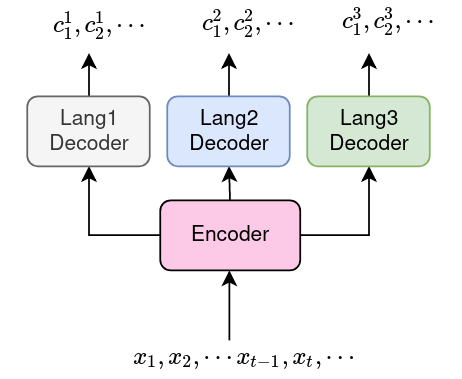
\includegraphics[width=0.5\textwidth]{fig/MultiTaskASR.png}
\end{frame}

\begin{frame}[t]{Multilingual Transfer Learning}
  However...\\
  Sometimes the model would overfitted on the source languages, and cannot adapt well on unseen target language.

  \vspace{1em}
  \pause
  Can we transfer the knowledge from source languages more effectively to unseen target language (under low-resource scenerio) ?

  \vspace{1em}

  \pause

  \center \textbf{Fast adaptation on unseen data}
\end{frame}

\begin{frame}[t]{Meta-Learning: Learning to Learn}
  Meta-Learning tries to solve \textbf{fast adaptation on unseen data}, \\
  and has gained some success in
  \begin{itemize}
    \item Computer Vision (\citealt{snell2017prototypical}, \citealt{rusu2018meta} ...)
    \item Machine Translation (\citealt{gu2018meta})
    \item Dialogue Generation (\citealt{mi2019meta})
    \item Speaker-Adaptative Training (\citealt{klejch2019speaker})
  \end{itemize}
\end{frame}

\section{Proposed Approach}
\begin{frame}
	\begin{center}
    %\weib{\LARGE{謝謝聆聽!}}
    \LARGE{Proposed Approach}
	\end{center}
\end{frame}

\begin{frame}[t]{Meta-Learning: Learning to Learn}
  We propose the multilingual training scheme based on the algorithm \textbf{Model-Agnostic Meta-Learning (MAML)} (\citealt{finn2017model}),

  \vspace{3em}

  In a nutshell,
  \begin{enumerate}
    \item Meta-training: Learn good \textbf{initialization} for adaptation by repeatedly simulating the learning process on source langauges
    \item Adaptation: use the learned initialization to adapt on target language
  \end{enumerate}
\end{frame}

\begin{frame}[t]{Model Architecture}
  \center 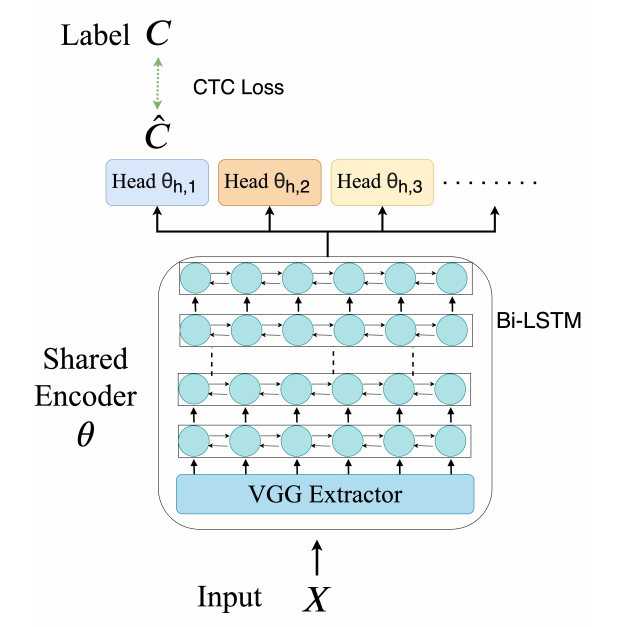
\includegraphics[width=0.55\textwidth]{fig/model_arch.png}
\end{frame}

\begin{frame}[t]{Formulation}
  Given a set of source langauges $\mathcal{D} = \{D_1, D_2, \cdots D_K \}$ and target language $D_t$
  \begin{equation*}
    \theta^{\star}_t, \theta^{\star}_{h,t} = \texttt{Learn}(D_t;\theta^{\star}) = \texttt{Learn}(D_t;\texttt{MetaLearn}(\mathcal{D})).
  \end{equation*}

\end{frame}

\begin{frame}[t]{Learn}
\begin{equation*}
  \begin{aligned}
    \theta^\prime, \theta^\prime_{h,t} = \texttt{Learn}(D_t;\theta^0) & = \arg \, \min_{\theta, \theta_{h,t}} \mathcal{L}_{D_t}(\theta, \theta_{h,t}) \\
  \end{aligned}
\end{equation*}
  \vspace{1em}

  $\mathcal{L}_{D_t}$: CTC loss on $D$

  \vspace{2em}
  Happened in 
  \begin{itemize}
    \item Language-specific learning in each meta-training episode
    \item Adaptation
  \end{itemize}
\end{frame}

\begin{frame}[t]{Meta-Learn}
  In each meta-training episode, we sample batch of tasks from $\mathcal{D}$, \\
  then sample two subsets from each task $k$ as train/test, $D^{tr}_k, D^{te}_k$.

  \begin{enumerate}
    \item Use $D^{tr}_k$ to simulate the learning process to obtain $\theta^\prime_k$, $\theta^\prime_{h,k}$
    \item Calculate the loss adapted on $D^{te}_k$, $\mathcal{L}_{D^{te}_k}(\theta^\prime_k, \theta^\prime_{h,k})$
    \item Meta-objective: $\mathcal{L}^{\text{meta}}_{\mathcal{D}}(\theta) =  \mathbb{E}_{k \sim \mathcal{D}} \; \mathbb{E}_{D_k^{tr}, D_k^{te}}$ $\Big [ \mathcal{L}_{D^{te}_k}(\theta^\prime_k, \theta^\prime_{h,k}) \Big ]$
    \item Use Gradient Descent to minimize $\mathcal{L}^{\text{meta}}_{\mathcal{D}}$ to obtain $\theta^\star$
  \end{enumerate}
  \pause
  \vspace{2em}
  \begin{equation*}
    \theta^{\star}_t, \theta^{\star}_{h,t} = \texttt{Learn}(D_t;\theta^{\star}) 
  \end{equation*}
\end{frame}

\section{Experimental Results}
\begin{frame}
	\begin{center}
    %\weib{\LARGE{謝謝聆聽!}}
    \LARGE{Experimental Results}
	\end{center}
\end{frame}

\begin{frame}[t]{Experimental Setting}
  Corpus: IARPA-BABEL (Conversational Telephone Speech)
  \begin{itemize}
    \item FLP: 40 $\sim$ 80 hr
    \item LLP: 10hr (subset of FLP)
  \end{itemize}
  \pause
  Languages:
  \begin{itemize}
    \item Source: Bengali (Bn), Tagalog (Tl), Zulu (Zu), Turkish (Tr), Lithuanian (Lt), Guarani (Gn)
    \item Target: Vietnamese (Vi), Swahili (Sw), Tamil (Ta), Kurmanji (Ku)
    \item Validation: Cross-validation
  \end{itemize}
\end{frame}

\begin{frame}[t]{CER on FLP}
  \center 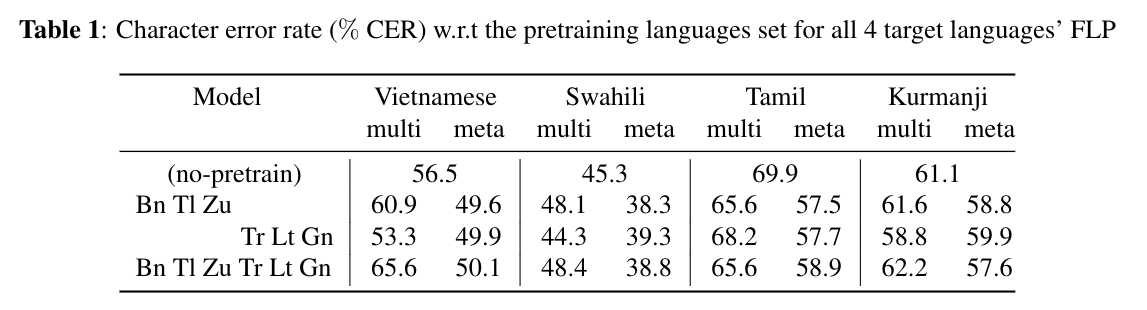
\includegraphics[width=1.0\textwidth]{fig/flp_table.png}
\end{frame}

\begin{frame}[t]{CER on LLP}
  \center 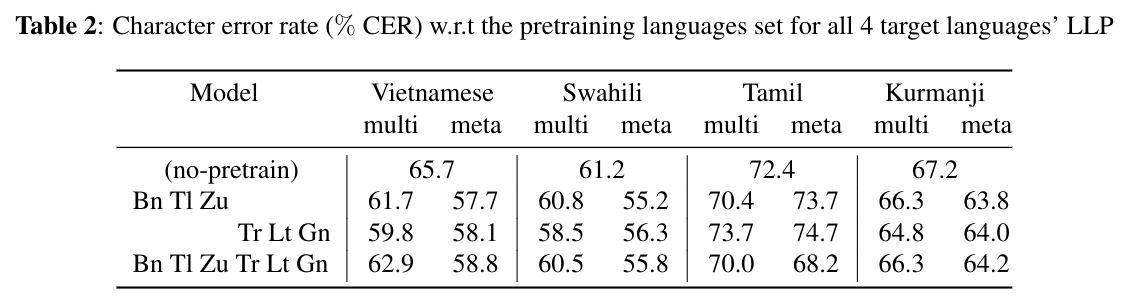
\includegraphics[width=1.0\textwidth]{fig/llp_table.png}
\end{frame}

\begin{frame}[t]{Learning Curve}
  \center 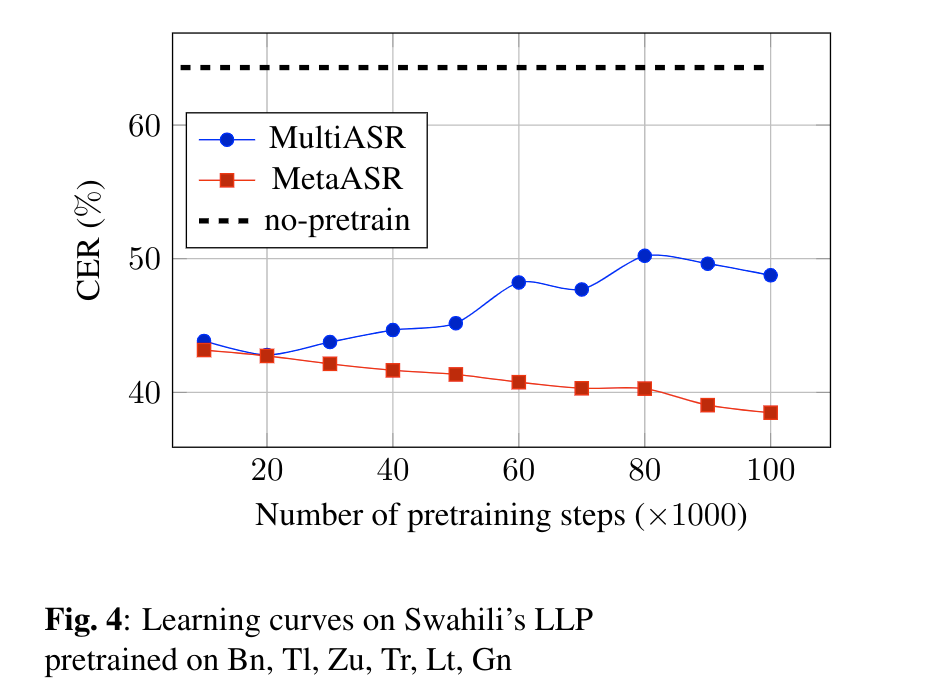
\includegraphics[width=0.7\textwidth]{fig/lr.png}
\end{frame}

\begin{frame}[t]{Conclusion}
  Meta-learned initialization
  \begin{itemize}
    \item overall performance is better than multitask-learned one
    \item doesn't overfit so easily
  \end{itemize}
  \pause
  \vspace{3em}
  \center new research direction for speech community
\end{frame}

%\begin{frame}[t]{Multi Transfer Learning (CER on LLP)}
  %Effect of pretraining step (Vietnamese for example)

    %\begin{figure}[H]
    %\centering
    %%\hspace{-5.2cm}
    %\begin{tikzpicture}[trim axis left, trim axis right]

    %\begin{axis}[
      %width=1.0\linewidth,
      %height=0.5\linewidth,
      %legend entries={PHN-near3, PHN-far3},
      %xlabel = {Number of pretraining steps ($\times 10^3$)},
          %xmin=-5,
          %xmax=200,
          %grid=both,
          %legend pos=inner north east,
          %ylabel={CER}]
    %\addplot+[smooth]table{stat/phn_near3};
    %\addplot+[smooth]table{stat/phn_far3};
    %\end{axis}
    %\end{tikzpicture}
  %\end{figure}

%\end{frame}

\begin{frame}
	\begin{center}
    \LARGE{Q\&A}
	\end{center}
\end{frame}

\bibliographystyle{plainnat}
\bibliography{M335}

\end{document} 
